Der Fit f�r U=40kV und A=10mA ist in Abb. \ref{fig:40_10_fit} zu sehen, die Fitparameter ergaben sich die Werte in Tabelle \ref{tab:40_10_fit}.

\begin{figure}[H]
	\centering
  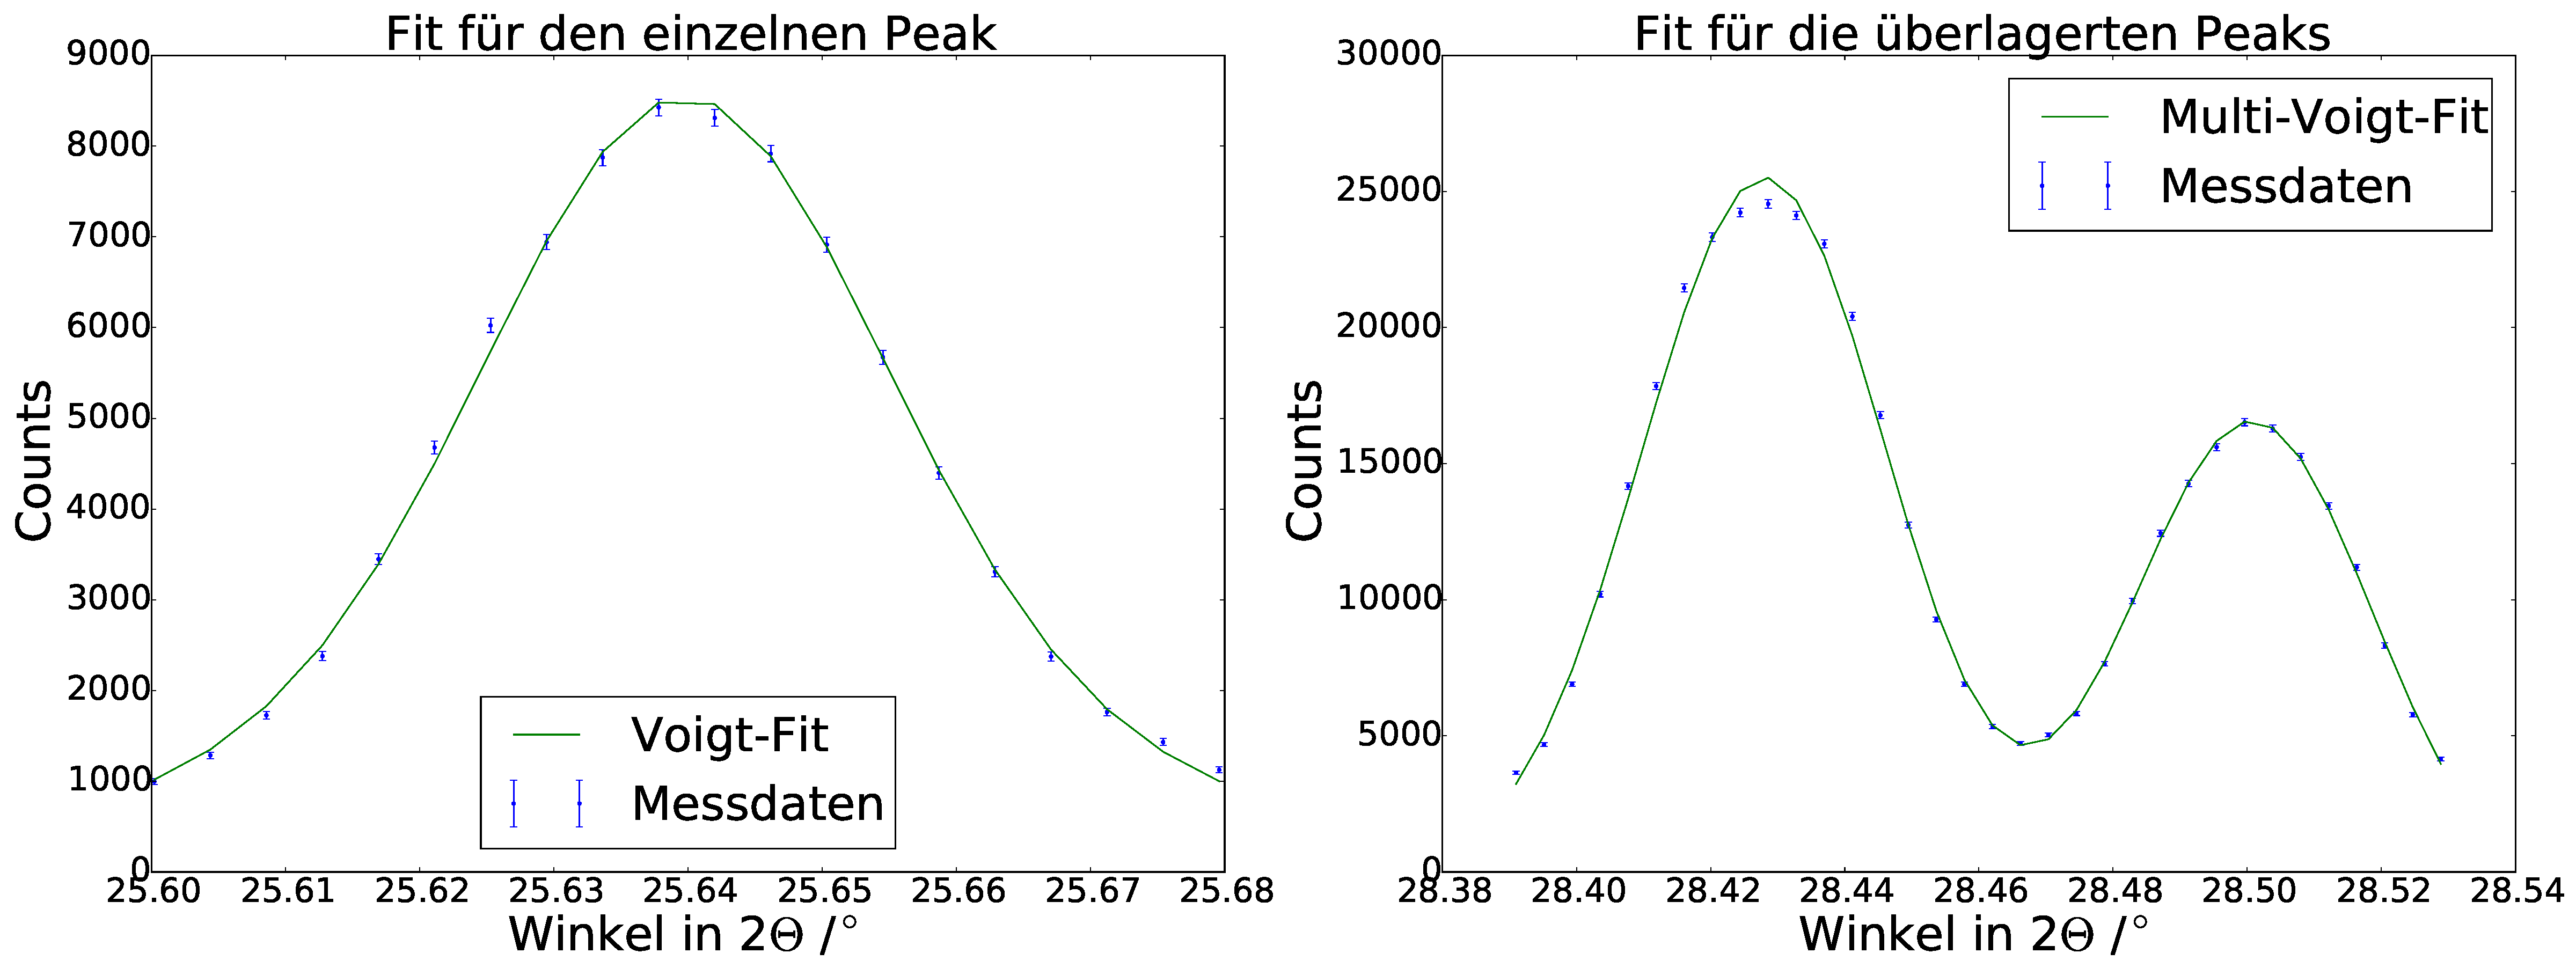
\includegraphics[scale=0.2]{40_10_voigt.pdf}
	\caption{Diffraktogramm bei 40kV Beschleunigungsspannung und einem Anodenstrom von 10mA}
	\label{fig:40_10_fit}
\end{figure}


\begin{table}[H]
\centering
\caption{Fitparameter f�r eine Beschleunigungsspannung von 40kV und einem Anodenstrom von 10mV}
\label{tab:40_10_fit}
\begin{tabular}{|c|c|c|c|c|c|c|}
\hline Peak & Paramter & Center & Amplitude & Sigma & Gamma & $\chi_{red}^2$ \\ 
\hline 1 & Wert & 25,6400 $\pm$ 0,0001 & 425 $\pm$ 6 & 0,0121 $\pm$ 0,0007 & 0,0089 $\pm$ 0,0007 & 4,11 \\ 
\hline 2 & Wert & 28,4282 $\pm$ 0,0003  & 1149 $\pm$ 52 & 0,018 $\pm$ 0,001 & 0,0007 $\pm$ 0,002 & 14,46 \\ 
\hline 3 & Wert & 28,5008 $\pm$ 0,0003 & 621 $\pm$ 75 & 0,020 $\pm$ 0,003 & -0,006 $\pm$ 0,006 & 14,46 \\ 
\hline 
\end{tabular} 
\end{table}


Der Fit f�r U=40kV und A=30mA ist in Abb. \ref{fig:40_30_fit} zu sehen, die Fitparameter ergaben sich die Werte in Tabelle \ref{tab:40_30_fit}.

\begin{figure}[H]
	\centering
  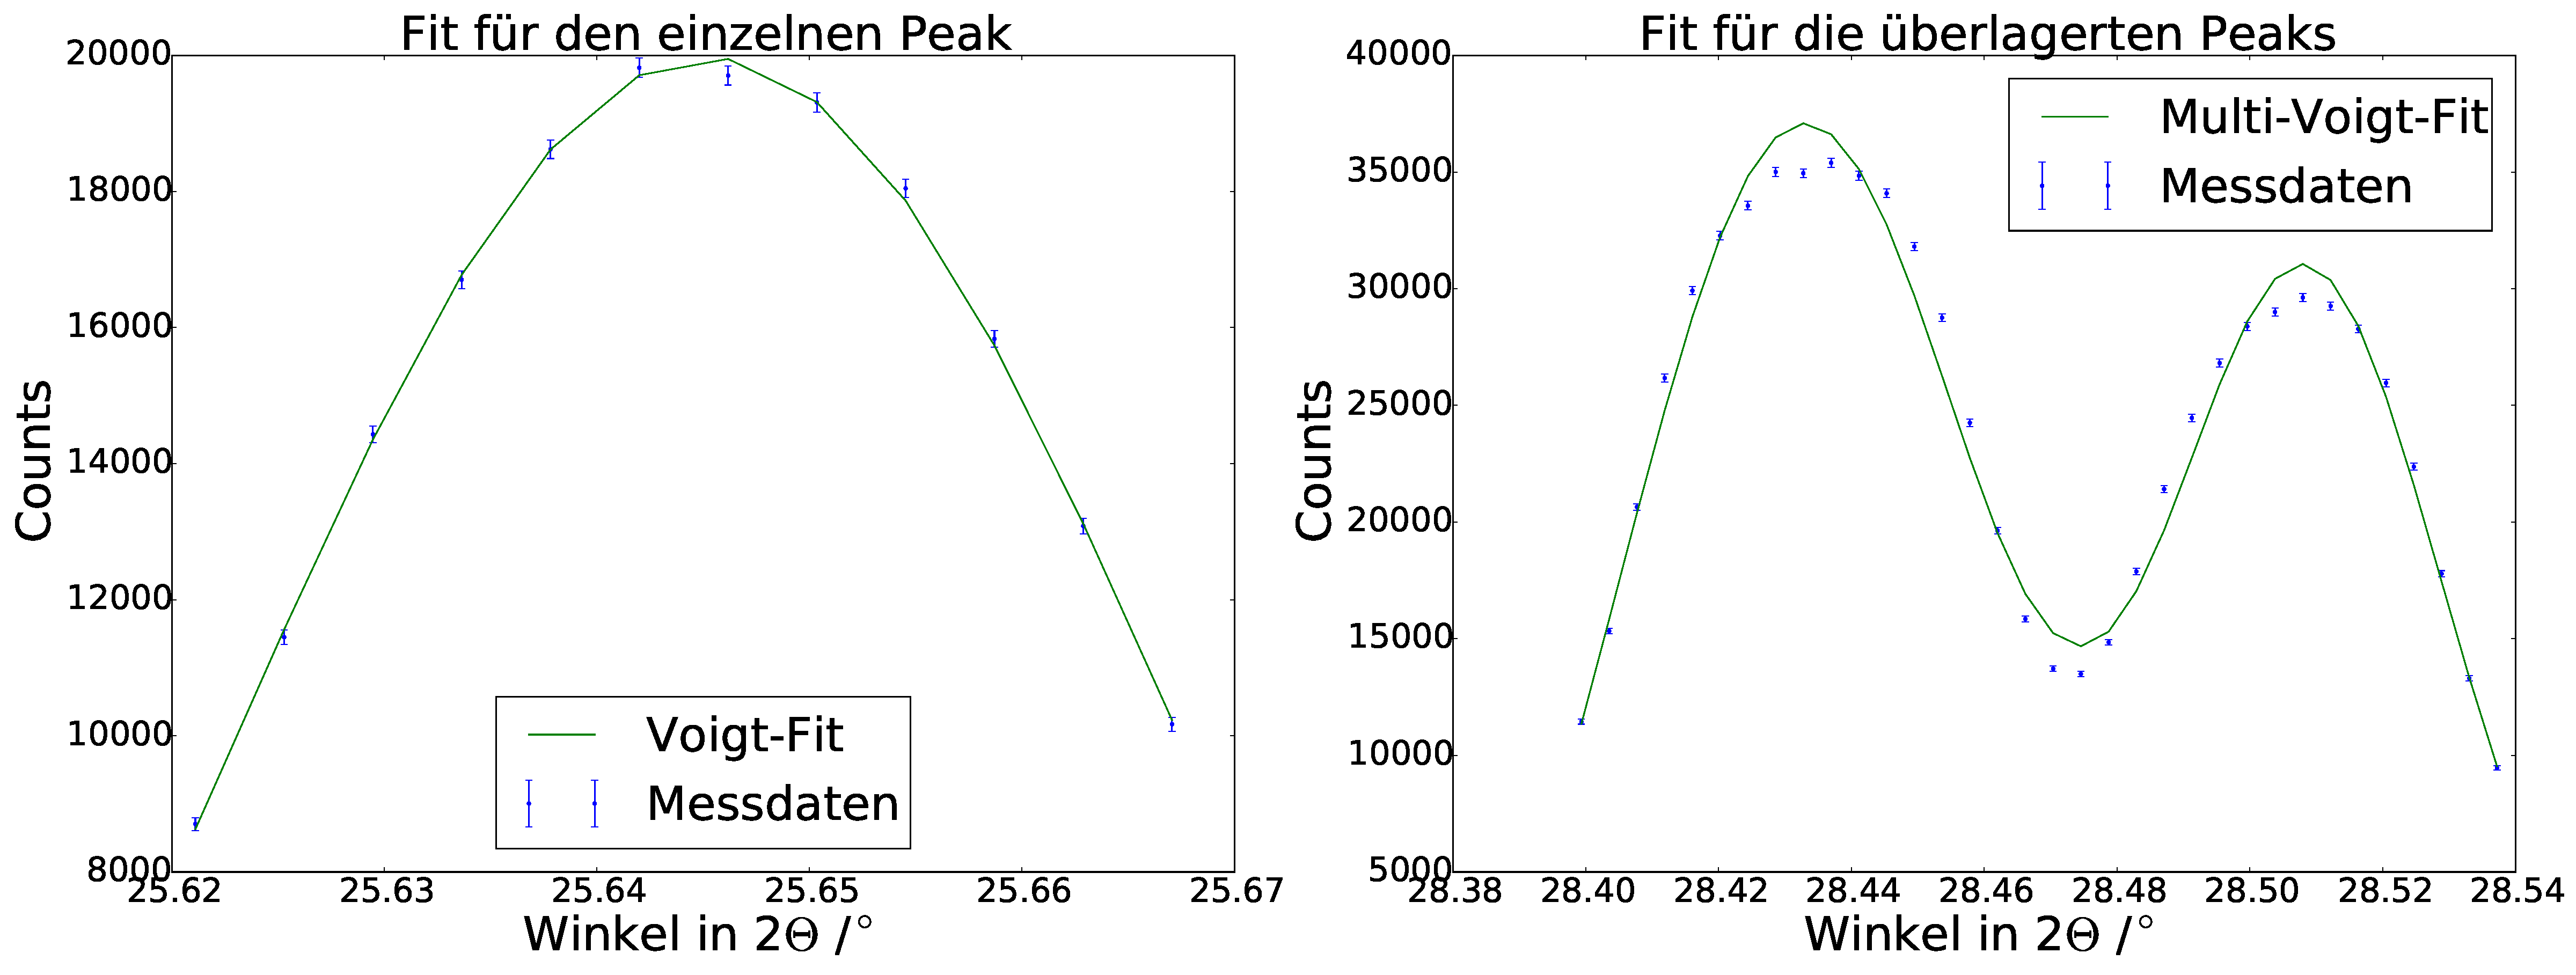
\includegraphics[scale=0.2]{40_30_voigt.pdf}
	\caption{Diffraktogramm bei 40kV Beschleunigungsspannung und einem Anodenstrom von 30mA}
	\label{fig:40_30_fit}
\end{figure}


\begin{table}[H]
\centering
\caption{Fitparameter f�r eine Beschleunigungsspannung von 40kV und einem Anodenstrom von 30mV}
\label{tab:40_30_fit}
\begin{tabular}{|c|c|c|c|c|c|c|}
\hline Peak & Paramter & Center & Amplitude & Sigma & Gamma & $\chi_{red}^2$ \\ 
\hline 1 & Wert & 25.64521 $\pm$ 0,00001 & 498 $\pm$ 158 & 0,031 $\pm$ 0,005 & -0,03 $\pm$ 0,02 & 1,13 \\ 
\hline 2 & Wert & 28,433 $\pm$ 0,001  & 1046 $\pm$ 873 & 0,01 $\pm$ 0,04 & -0,05 $\pm$ 0,05 & 71,49 \\ 
\hline 3 & Wert & 28,507 $\pm$ 0,001 & 1814 $\pm$ 613 & 0,022 $\pm$ 0,005 & -0,004 $\pm$ 0,012 & 71,49 \\ 
\hline 
\end{tabular} 
\end{table}
